% move all configuration stuff into one file so we can focus on the content
\documentclass[aspectratio=169,hyperref={pdfpagelabels=false,colorlinks=true,linkcolor=white,urlcolor=blue},t]{beamer}

%%%%%%%%%%%%%%%%%%%%%%%%%%%%%%%%%%%%%%%%%%%%%%%%%%%%%%%%%%%%%%%%%%%%%%%%%%%%%%%%%%
%%%%%%%%%%%%%%%%%%%%%%%%%%%%%%%%%%%%%%%%%%%%%%%%%%%%%%%%%%%%%%%%%%%%%%%%%%%%%%%%%%
% packages
\usepackage{pict2e}
\usepackage{epic}
\usepackage{amsmath,amsfonts,amssymb}
\usepackage{units}
\usepackage{fancybox}
\usepackage[absolute,overlay]{textpos} 
\usepackage{media9} % avi2flv: "C:\Program Files\ffmpeg\bin\ffmpeg.exe" -i TuneFreqFilterbank.avi -b 600k -s 441x324 -r 15 -acodec copy TuneFreqFilterbank.flv
\usepackage{animate}
\usepackage{gensymb}
\usepackage{multirow}
\usepackage{silence}
\usepackage[backend=bibtex,style=ieee]{biblatex}
\AtEveryCitekey{\iffootnote{\tiny}{}}
\addbibresource{references}

%%%%%%%%%%%%%%%%%%%%%%%%%%%%%%%%%%%%%%%%%%%%%%%%%%%%%%%%%%%%%%%%%%%%%%%%%%%%%%%%%%
%%%%%%%%%%%%%%%%%%%%%%%%%%%%%%%%%%%%%%%%%%%%%%%%%%%%%%%%%%%%%%%%%%%%%%%%%%%%%%%%%%
% relative paths
\graphicspath{{graph/}}


%%%%%%%%%%%%%%%%%%%%%%%%%%%%%%%%%%%%%%%%%%%%%%%%%%%%%%%%%%%%%%%%%%%%%%%%%%%%%%%%%%
%%%%%%%%%%%%%%%%%%%%%%%%%%%%%%%%%%%%%%%%%%%%%%%%%%%%%%%%%%%%%%%%%%%%%%%%%%%%%%%%%%
% units
\setlength{\unitlength}{1mm}

%%%%%%%%%%%%%%%%%%%%%%%%%%%%%%%%%%%%%%%%%%%%%%%%%%%%%%%%%%%%%%%%%%%%%%%%%%%%%%%%%%
%%%%%%%%%%%%%%%%%%%%%%%%%%%%%%%%%%%%%%%%%%%%%%%%%%%%%%%%%%%%%%%%%%%%%%%%%%%%%%%%%%
% theme & layout
\usetheme{Frankfurt}
\beamertemplatenavigationsymbolsempty
%\setbeamertemplate{frametitle}[smoothbars theme]
\setbeamertemplate{frametitle}
{
    \begin{beamercolorbox}[ht=1.8em,wd=\paperwidth]{frametitle}
        \vspace{-.1em}%
        \hspace{.2em}{\strut\insertframetitle\strut}
        
        \hspace{.2em}\small\strut\insertframesubtitle\strut
        %\hfill
        %
\includegraphics[height=.8cm,keepaspectratio]{CenterMusicTechnology-solid-2lines-white-CoAtag}
        
    \end{beamercolorbox}
    \begin{textblock*}{100mm}(11.6cm,.7cm)
        \includegraphics[height=.8cm,keepaspectratio]{logo_GTCMT_black}
    \end{textblock*}
}

% set this to ensure bulletpoints without subsections
\usepackage{remreset}
\makeatletter
\@removefromreset{subsection}{section}
\makeatother
\setcounter{subsection}{1}

%---------------------------------------------------------------------------------
% appearance
\setbeamercolor{structure}{fg=gtgold}
\setbeamercovered{transparent} %invisible
\setbeamercolor{bibliography entry author}{fg=black}
\setbeamercolor*{bibliography entry title}{fg=black}
\setbeamercolor*{bibliography entry note}{fg=black}

%\usepackage{pgfpages}
%\setbeameroption{show notes}
%\setbeameroption{show notes on second screen=right}
%---------------------------------------------------------------------------------
% fontsize
\let\Tiny=\tiny

%%%%%%%%%%%%%%%%%%%%%%%%%%%%%%%%%%%%%%%%%%%%%%%%%%%%%%%%%%%%%%%%%%%%%%%%%%%%%%%%%%
%%%%%%%%%%%%%%%%%%%%%%%%%%%%%%%%%%%%%%%%%%%%%%%%%%%%%%%%%%%%%%%%%%%%%%%%%%%%%%%%%%
% warnings
\pdfsuppresswarningpagegroup=1
\WarningFilter{biblatex}{Patching footnotes failed}
\WarningFilter{latexfont}{Font shape}
\WarningFilter{latexfont}{Some font shapes}
\WarningFilter{gensymb}{Not defining}



\subtitle{Part 6.4: amendment: Introduction to NMF}

%%%%%%%%%%%%%%%%%%%%%%%%%%%%%%%%%%%%%%%%%%%%%%%%%%%%%%%%%%%%%%%%%%%%%%%%%%%%
\begin{document}
    % generate title page
	

\begin{frame}
    \titlepage
    %\vspace{-5mm}
    \begin{flushright}
        \href{http://www.gtcmt.gatech.edu}{\includegraphics[height=.8cm,keepaspectratio]{logo_GTCMT_black}}
    \end{flushright}
\end{frame}


    \section[overview]{lecture overview}
        \begin{frame}{introduction}{overview}
            \begin{itemize}
                \item   \textbf{additional reading}  
                    \begin{itemize}
                        \item   D. D. Lee and H. S. Seung, \textit{Algorithms for Non-negative Matrix Factorization}, NIPS, 2001
                        \item   P. Smaragdis and J. C. Brown, \textit{Non-negative Matrix Factorization for Polyphonic Music Transcription}, WASPAA, 2003
                        \item   A. Cichocki, R. Zdunek, A. H. Phan and S. Amari, \textit{Non-negative Matrix and Tensor Factorization: applications to exploratory multi-way data analysis and blind source separation}, John Wiley \& Sons, 2009
                    \end{itemize}
                \bigskip
                \item<2->   \textbf{lecture content}
                    \begin{itemize}
                        \item   what is nmf?
                        \item   objective function
                        \item   update rules
                        \item   penalty terms
                        \item   exercise
                    \end{itemize}
            \end{itemize}
        \end{frame}
   
    \section[what is nmf]{what is nmf}
        \begin{frame}{what is nmf?}{problem description}
            \begin{itemize}
                \item   \textbf{Non-negative Matrix Factorization (NMF)}\\
                Given a $m \times n$ matrix $V$, find a $m \times r$ matrix $W$ and a $r \times n$ matrix $H$ such that
                \begin{equation*}
                V \approx WH
                \end{equation*}
                \begin{itemize}
                		\item all matrices must be non-negative
                		\item rank $r$ is usually smaller than $m$ and $n$
                \end{itemize}
              		                
                \bigskip
                \item<2->   \textbf{advantage of non-negativity?}
                    \begin{itemize}
                        \item<2->   additive model
                        \item<3->   relates to probability distributions
                        \item<4->   efficiency?
                    \end{itemize}
            \end{itemize}
        \end{frame}    
        
        \begin{frame}{what is nmf?}{basic nmf model}
            \begin{itemize}
                \item  The NMF model can also be expressed like this:\footfullcite{cichocki_nmf_2009}\\
                \begin{equation*}
                V = \sum_{i = 1}^r w_{i} \cdot h_{i} + E
                \end{equation*}
			    \begin{itemize}
					\item  $V \in \mathbb{R}^{m \times n}$
					\item  $W = [w_{1}, w_{2}, ..., w_{r}] \in \mathbb{R}^{m \times r}$
					\item  $H  = [h_{1}, h_{2}, ..., h_{r}]^{T} \in \mathbb{R}^{r \times n}$
					\item  $E$ is the error matrix													   
				\end{itemize}			                   
                         
                \bigskip
                \item  visualization
                \begin{figure}
                		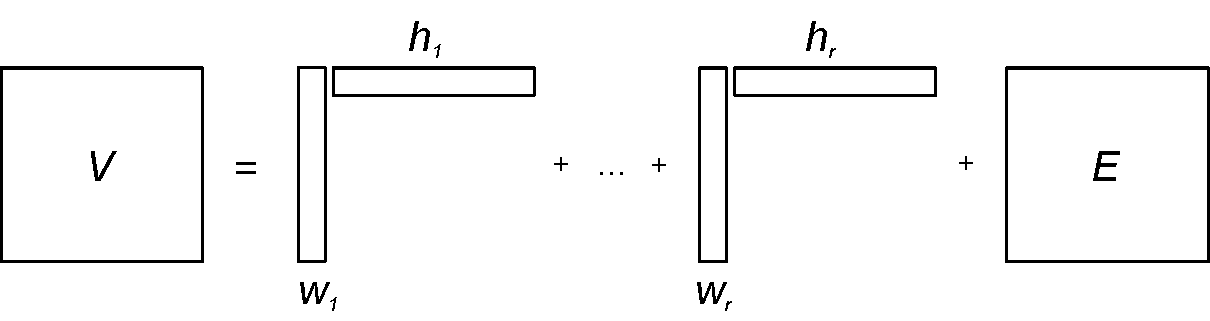
\includegraphics[scale=.35]{Nmf_Decomposition}
                \end{figure}
            \end{itemize}
        \end{frame}        
        
    \section[objective function]{objective function}
        \begin{frame}{objective function}{distance and divergence}
        minimize the distance $D(V || WH)$,  typical distance measures:\\
        
           \begin{itemize}
                \item  squared Euclidean distance:\\
                \begin{equation*}
                \parallel A - B\parallel^{2} = \sum_{i j} (A_{i j} - B_{i j})^{2}
                \end{equation*}
			   \item  generalized K-L divergence:\\
			   \begin{equation*}
                D( A \parallel B) = \sum_{i j} (A_{i j} log\frac{A_{i j}}{B_{i j}} - A_{i j} + B_{i j})
                \end{equation*}		                
                \bigskip
                \item<2-> others\footfullcite{cichocki_nmf_2009}: Bregman Divergence, Alpha-Divergence, Beta-Divergence, ... etc.
           \end{itemize}
        \end{frame}          
    
    \section[update rules]{update rules}
        \begin{frame}{update rules}{cost function and gradient descent}
            \begin{itemize}
                \item \textbf{example}: squared Euclidean distance
                   \begin{itemize} 
                        \item  cost function $J = \parallel V - WH\parallel^{2}$
                   \end{itemize}			   			   

               \item<2->  \textbf{optimization--- gradient descent}: \href{https://en.wikipedia.org/wiki/Gradient_descent}{\underline{\textit{wikipedia page}}}
                       \begin{itemize}
                            \item  given a function $f(x_{1}, x_{2})$, find the minimum $x_{1} = a$ and $x_{2} = b$
                            \item  initialize $x_{i}(0)$ with random numbers
                            \item  update points iteratively:  
                                     \begin{equation*}
                                         x_{i}(n+1) = x_{i}(n) - \alpha \cdot \frac{\partial f}{\partial x_{i}},  i = [1, 2]
                                     \end{equation*}
                            \item[$\Rightarrow$] as iteration number $n$ increases, $x_{1}$, $x_{2}$ will be closer to $a$, $b$.
                       \end{itemize}			   			   
            \end{itemize}
        \end{frame}    
          
        \begin{frame}{update rules}{additive vs multiplicative} 
           NMF, cost function $J = \parallel V - WH\parallel^{2}$\\ How to optimize it? \footfullcite{seung_nmf_2001}
           \begin{itemize}
                \item  \textbf{additive} update rules:
                \begin{equation*}
                H \leftarrow H + \alpha \frac{\partial J}{\partial H} = H + \alpha [(W^{T}V) - (W^{T}WH)]
                \end{equation*}
                \begin{equation*}
                W \leftarrow W + \alpha \frac{\partial J}{\partial W} = W + \alpha [(VH^{T}) - (WHH^{T})]
                \end{equation*}
			   \item  \textbf{multiplicative} update rules:
                \begin{equation*}
                H \leftarrow H \frac{(W^{T}H)}{(W^{T}WH)}
                \end{equation*}
                \begin{equation*}
                W \leftarrow W \frac{(VH^{T})}{(WHH^{T})}
                \end{equation*}
           \end{itemize}
        \end{frame}        
    
    \section[penalty terms]{penalty terms}
        \begin{frame}{penalty terms}{additional constraints to the cost function}
            \begin{itemize}
                \item   additional penalty terms (regularization terms) may be added to the cost function (e.g., sparsity in $W$ or $H$)
            \end{itemize}
            \begin{equation*}
                J = \parallel V - WH\parallel^{2} + \alpha J_\mathrm{W}(W) + \beta J_\mathrm{H}(H)
            \end{equation*}
            \begin{itemize}
                \item $\alpha,\beta$: coefficients for controlling degree of sparsity
                \item $J_\mathrm{W}$ and $J_\mathrm{H}$: typically $L_{1},L_{2}$ norm 
            \end{itemize}
        \end{frame}
              
    \section[exercise]{in class exercise}
        \begin{frame}{in class exercise}{nmf for music transcription}
        \matlabexercise{nmf based pitch tracking}
            \begin{itemize}
                \item   \textbf{unsupervised}  
                    \begin{itemize}
                        \item   read audio file \textit{4notes\_train.wav}
                        \item   compute magnitude spectrogram using \textit{spectrogram( )}
                        \item   compute matrix W and H using \textit{nnmf( )}
                        \item   visualize the templates and activations
                    \end{itemize}
                \bigskip
                \item   \textbf{supervised}
                    \begin{itemize}
                        \item   read audio file \textit{2notes\_test.wav}  
                        \item   compute magnitude spectrogram using \textit{spectrogram( )}
                        \item   get H2 using [W2, H2] = PfNmf(Y, W, [ ], [ ], [ ], 0, 0)
                        \item   visualize the activations and plot the error curve
                    \end{itemize}
            \end{itemize}
        \end{frame}
        
        \begin{frame}{in class exercise}{expected results}
        %\matlabexercise{nmf based pitch tracking}
        resulting templates 
			\begin{figure}      
         		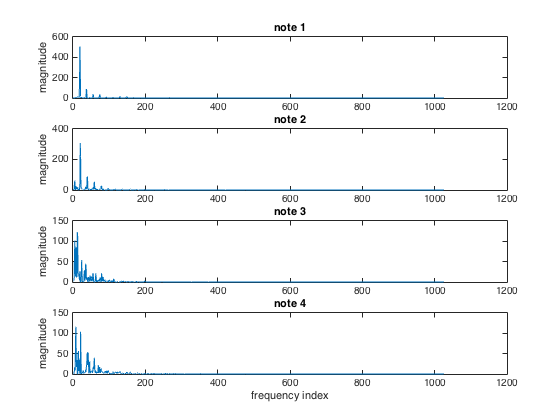
\includegraphics[scale=.45]{Nmf_ExerciseDictionary}
			\end{figure}        
        \end{frame}
        
        \begin{frame}{in class exercise}{expected results}
        %\matlabexercise{nmf based pitch tracking}
		resulting activations
			\begin{figure}
				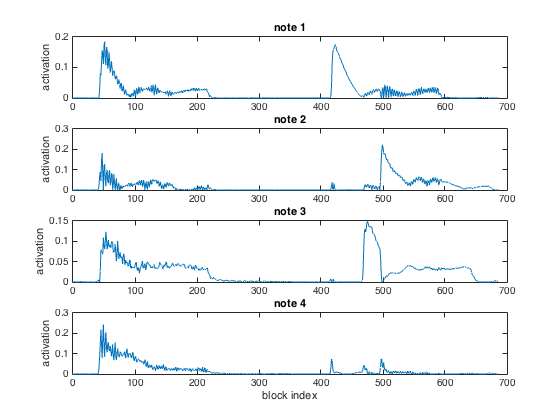
\includegraphics[scale=.45]{Nmf_ExerciseActivation}
			\end{figure}
        \end{frame}         
         
        \begin{frame}{in class exercise}{expected results}
        %\matlabexercise{nmf based pitch tracking}
		resulting error curve
			\begin{figure}
				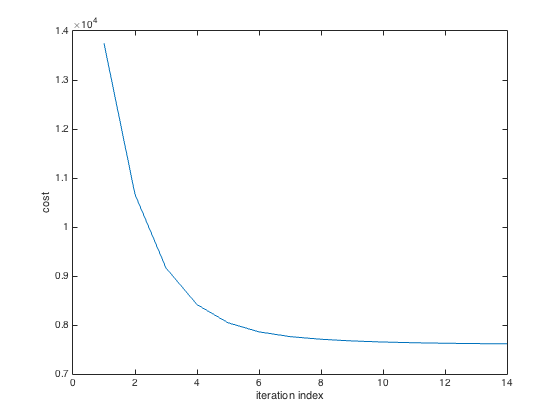
\includegraphics[scale=.45]{Nmf_ExerciseError}
			\end{figure}
        \end{frame}  

\end{document}

